% 2017 山东卷（文）第21题 题图：单圆锥曲线与少量直线
% 椭圆 x^2/4 + y^2/2 = 1，圆 N 过 O，动直线 l: y = 7x/8 + 15/8
% A,B 为 l 与椭圆的交点，D 为 AB 中点，DE,DF 为 D 到圆 N 的两条切线
\usetikzlibrary{arrows.meta}
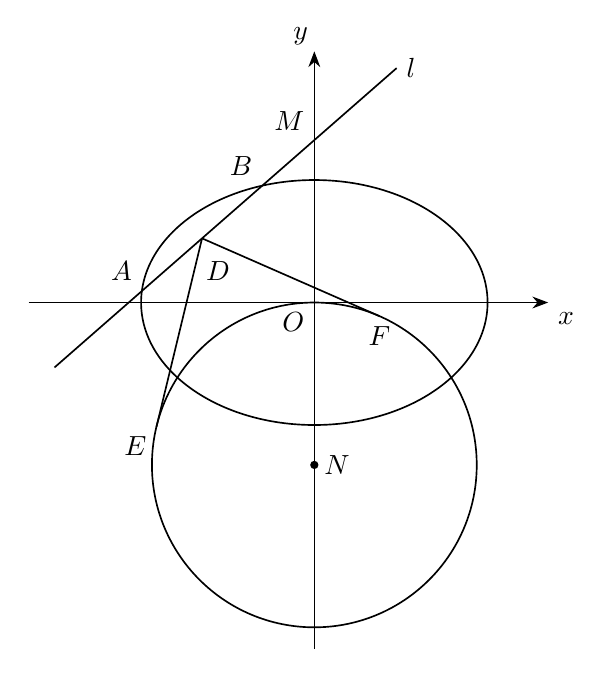
\begin{tikzpicture}[x=1.1cm,y=1.1cm,line width=.6pt,font=\normalsize,>=Stealth]
\def\ellA{2.00000000}
\def\ellB{1.41421356}
\def\circR{1.87500000}
\coordinate (O) at (0.00000000,0.00000000);
\coordinate (M) at (0.00000000,1.87500000);
\coordinate (N) at (0.00000000,-1.87500000);
\coordinate (A) at (-1.99117271,0.13272388);
\coordinate (B) at (-0.60141989,1.34875760);
\coordinate (D) at (-1.29629630,0.74074074);
\coordinate (E) at (-1.82243087,-1.43412503);
\coordinate (F) at (0.75295586,-0.15782719);
\coordinate (Llow) at (-3.00000000,-0.75000000);
\coordinate (Lhigh) at (0.95000000,2.70625000);
\draw[->] (-3.30000000,0.00000000)--(2.70000000,0.00000000) node[below right] {$x$};
\draw[->] (0.00000000,-4.00000000)--(0.00000000,2.90000000) node[anchor=south east,inner sep=0pt,xshift=-2pt,yshift=2pt] {$y$};
\draw (O) ellipse ({\ellA} and {\ellB});
\draw (N) circle ({\circR});
\draw (Llow)--(Lhigh);
\draw (D)--(E);
\draw (D)--(F);
\fill (N) circle (1.5pt);
\node[below left] at (O) {$O$};
\node[above left] at (M) {$M$};
\node[right] at (N) {$N$};
\node[above left] at (A) {$A$};
\node[above left] at (B) {$B$};
\node at (-1.11200000,0.36400000) {$D$};
\node[below left] at (E) {$E$};
\node[below] at (F) {$F$};
\node[right] at (Lhigh) {$l$};
\end{tikzpicture}
